%!TEX encoding = UTF-8 Unicode
%!TEX TS-program = pdflatex

%%% --- PREAMBLE --- %%%
\documentclass[a4paper,11pt]{article}

\usepackage[italian]{babel}
\usepackage[left=2cm,right=2cm,top=2cm,bottom=2cm,headheight=14pt]{geometry}
\usepackage[T1]{fontenc} % OT1: basic, T1: western, T3 and T5: exotic, T4: lots of characters but WORSE READABILITY
\usepackage[utf8x]{inputenc} % utf8x supports more characters than utf8
\usepackage{graphicx} % import PNG, JPG and PDF with \includegraphics
\usepackage[usenames,table]{xcolor} % \color
\usepackage{amssymb}
\usepackage{amsmath}
\usepackage{amsfonts}
\usepackage{float}
\usepackage{mathtools} % (!! PLACE BEFORE hyperref !!)
\usepackage{xfrac} % \sfrac
\usepackage{cancel} % \cancel \cancelto
\usepackage{hyperref} % interactive links in TOC, URLs and references
% unneded \usepackage{fixltx2e} % provides \textsubscript and makes some fixes
\usepackage[toc,page]{appendix}
\usepackage{siunitx} % \num \si \SI
\usepackage{alltt} % {alltt} (like verbatim but with commands)
\usepackage{moreverb} % {listing}
\usepackage{listings} % {lstlisting}
\usepackage[overload]{textcase} % fixes \MakeUppercase and \MakeLowercase
\usepackage[normalem]{ulem} % \uline \uwave \sout \xout
\usepackage{enumerate} % adds options for {enumerate}
\usepackage{paralist} % inline lists with {inparaenum}
\usepackage[official]{eurosym} % \euro
\usepackage{tabu} % {tabu} (like {tabular} with improvements)
\usepackage{layout} % layout description
\usepackage{multicol} % {multicols}
\usepackage{lipsum} % filling text generator with \lipsum
\usepackage[section]{placeins} % inhibits float figures from trepassing a section boundary
\usepackage{subfig} % \subfloat to be used inside {figure}
\usepackage{wrapfig} % {wrapfigure} (like {figure} but allows text to flow on its sides)
\usepackage{ifthen} % \ifthenelse
\usepackage{calc}
\usepackage{array}
\usepackage{multirow}
\usepackage{booktabs} % \toprule, \midrule, \bottomrule
\usepackage{fancyhdr}
\usepackage{wasysym}
\graphicspath{ {../Figs-Tabs/} } % graphics search directories
\setcounter{tocdepth}{1} % -1: part, 0: chapter, 1: section, 2: subsection, 3: subsubsection

\lstset{ %
	language=C,
	deletekeywords={},
	morekeywords={},
	backgroundcolor=\color{white},
	basicstyle=\ttfamily\small,
	commentstyle=\color{teal},
	keywordstyle=\color{magenta},
	stringstyle=\color{purple},
	identifierstyle=\color{violet!80!black},
	numbers=left,
	numbersep=7pt,
	numberstyle=\scriptsize\sffamily\color{gray},
	stepnumber=1,
	breakatwhitespace=false,
	breaklines=true,
	keepspaces=true,
	showspaces=false,
	showstringspaces=false,
	showtabs=false,
	tabsize=2,
	captionpos=none,
}

\newcommand{\ndr}[1]{\footnote{#1 (n.d.r.)}}

\newcommand{\fig}[1]{\figurename{ \ref{fig:#1}}} %inserting reference to figures
\newcommand{\tab}[1]{\tablename{ \ref{tab:#1}}} % inserting reference to tables
\newcommand{\eqn}[1]{equazione \eqref{eq:#1}} % inserting reference to equation

\newcommand{\dof}{\text{ dof}} % degrees of freedom
\newcommand{\paral}{\mathbin{\|}} % impedance parallel
\DeclareSIUnit\deca{decade} % decade unit definition for use in siunitx
\DeclareSIUnit\gauss{Gs} % Gauss unit definition for use in siunitx

\newcommand{\insertpart}[2]{\input{#1}}
\newcommand{\e}{\textbf{$e^{-}$}}

\sisetup{%
	separate-uncertainty = true,
	per-mode = symbol,
	bracket-numbers = false,
	multi-part-units = single,
	table-number-alignment = center,
	range-phrase = \text{--},
	range-units = single,
	output-complex-root =  \text{\ensuremath{j}},
	table-figures-decimal = 3,
	table-figures-exponent = 0,
	table-figures-integer = 2,
	table-figures-uncertainty = 2,
}

%%% --- DOCUMENT --- %%%


%%%%% SIunits example use:
% \si{\kilo\volt\per\meter\squared} -> kV/m^2
% \SI{1.222 (34)}{\joule\second}    -> 1.222 +- 0.034 Js
% \SI{1.222 \pm 0.034}{\nF}         -> 1.222 +- 0.034 nF
% use it plz

\pagestyle{fancy}
\author{Gruppo BF \\ Thomas Giannoni, Valerio Lomanto, Roberto Ribatti}
\title{Esercitazione N. 12: Flip-Flop e contatori}
\date{4 aprile 2017}

\author{Gruppo BF \\ Thomas Giannoni, Valerio Lomanto, Roberto Ribatti}
\title{Esercitazione N. 12: Flip-Flop e contatori}
\date{4 aprile 2017}

\begin{document}
\maketitle
\begin{abstract}
L'obiettivo dell'esperienza è la realizzazione e l'analisi di semplici circuiti logici sequenziali, in particolare: un FLIP-FLOP D-LATCH, divisori di frequenza binari, uno shift register con D-Latch e generatore di sequenze pseudo-casuali (linear feedback shift register).
\end{abstract}

\section{Misura delle caratteristiche di IC SN74LS244 }
\subsection{Caratteristiche statiche}
	Per tutta la sezione si è proceduto ad alimentare il circuito con una tensione di alimentazione $V_{cc} =$\SI{5.01 \pm 0.03}{\volt}.
	\paragraph{Misure delle tensioni d'operazione}
	Per effettuare la misura delle tensioni operative di una porta NOT si 
	è montato il circito in \figurename{ \ref{f:c1}}
		\begin{figure}[h]
			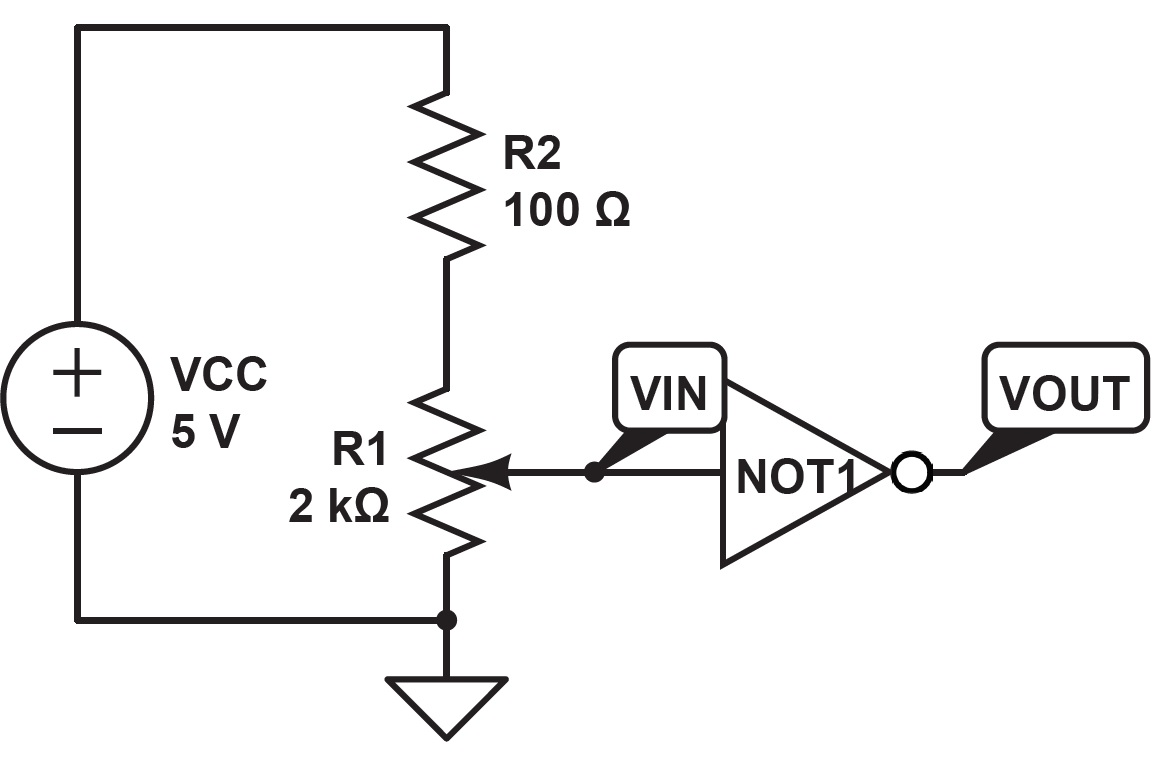
\includegraphics[scale=1.0]{../Figs-Tabs/immagine1.png}
			\caption{Rappresentazione del primo circuito impiegato.}
			\label{f:c1}
		\end{figure} ,
	dopodiché si è andati a  campionare la tensione in uscita, $V_{out}$, in funzione della tensione di ingresso , $V_{in}$.
	
	Il circuito in  \figurename{ \ref{f:c1}} permette la variazione di  $V_{in}$ variando la resistenza del trimmer $R_{1}$;infatti esso  rappresenta un partitore di tensione.
	
		Per la costruzione circuitale sono state impiegate: un trimmer $R_{1}$ di valore massimale $R_{1}^{max}=$\SI{94.0 \pm 0.8 }{\kilo \ohm} ed na resistenza $R_{2}=$\SI{100.8 \pm 0.9 }{ \ohm}.
		
	Si riportano i dati campionati in \tablename{ \ref{t:1}}
		\begin{table}[hb]
		\centering
		\begin{tabular}{|s|s|}
			\toprule
			V_{in} [\si{\volt}] & 	V_{out} [\si{\volt}]\\
			\midrule
		 0	\pm 1e-3 & 4.38 \pm 0.02\\
			0.265 \pm 0.002 & 4.23 \pm 0.02\\
			0.584 \pm 0.003 & 4.02 \pm 0.02\\
			0.780 \pm 0.004 & 3.87 \pm 0.02\\
			0.881 \pm 0.005 & 3.78 \pm 0.02\\
			0.945 \pm 0.005 & 3.44 \pm 0.02\\
			1.003 \pm 0.005 & 2.95 \pm 0.02\\
			1.065 \pm 0.006 & 2.01 \pm 0.01\\
			1.103 \pm 0.008 & 0.1773 \pm 0.009\\
			1.238 \pm 0.009 & 0.1728 \pm 0.009\\
			1.56 \pm 0.01 & 0.1728 \pm 0.009\\
			1.775 \pm 0.02 & 0.1728 \pm 0.009\\
			1.991 \pm 0.02 & 0.1727 \pm 0.009\\
			2.52 \pm 0.02 & 0.1727 \pm 0.009\\
			3.02 \pm 0.02 & 0.1726 \pm 0.009\\
			3.48 \pm 0.02 & 0.1726 \pm 0.009\\
			3.93 \pm 0.02 & 0.1726 \pm 0.009\\
			5.00 \pm 0.03 & 0.1726 \pm 0.009\\
			\bottomrule
		\end{tabular}
		\caption{Si riportano i valori corrispondenti alle nostre acquisizioni.I dati campionati sono stati ottenti col multimetro digitale.
		Si è associato alle misure l'incertezza di un  digit sulla prima cifra che risultasse instabile sommata in quadratra con eventali errori di calibrazione del mltimetro.}
		\label{t:1}
	\end{table}
	.
	Effettando un grafico  ( \figurename{ \ref{f:i1}} )
	 dei dati in  \tablename{ \ref{t:1}}, ( a cui sono stati scorporati gli errori di calibrazione del multimetro essendo uniformi per le scale impiegate) si osservano i valori di :\\
	 $V_{I,H}$, tensione in ingresso associata all'uscita HIGH;\\
	 $V_{I,L}$, tensione in ingresso associata all'uscita LOW;\\
	 $V_{O,H}$, tensione in uscita  associata all'uscita HIGH;\\
	 $V_{O,L}$, tensione in uscita associata all'uscita LOW.\\
	 
	 Essendo tali valori da intendersi come intervalli di tensione si sono osservati i loro valori superiori ed inferiori ottenendo :
	 \begin{center}
	 $V_{I,H}^{max}\sim$\SI{0}{\volt} \\
	 $V_{I,H}^{min}=$\SI{1.003 \pm 0.005}{\volt}\\
	 $V_{I,L}^{max}=$\SI{5.00 \pm 0.03}{\volt}\\
	 $V_{I,L}^{min}=$\SI{1.108 \pm 0.008}{\volt}\\
	 
	 $V_{O,H}^{min}=$\SI{2.95 \pm 0.02}{\volt}\\
	 $V_{O,H}^{max}=$\SI{4.38 \pm 0.02}{\volt}\\
	 $V_{O,L}^{min}=$\SI{0.1726 \pm 0.0009}{\volt}\\
	 $V_{O,L}^{max}=$\SI{0.1773 \pm 0.0009}{\volt}	\\
	 \end{center}
	 
	 Tali stime risultano essere meno restrittive dei  valori
	  forniti dal costruttore nel datasheet:
	   \begin{center}
	  	
	  	$V_{O,H}^{min,atteso}=$\SI{2.4}{\volt}\\
	  	$V_{O,L}^{max,atteso}=$\SI{0.4}{\volt}\\
	  	$V_{I,H}^{min,atteso}=$\SI{2}{\volt}\\
	  	$V_{I,L}^{max,atteso}=$\SI{0.8}{\volt}.\\
	  \end{center}
	  Si imputa che questa lieve discrepanza 
	 con i valori attesi, sia dovuta al fatto che essi siano misurati nelle peggiori condizioni di operatività possibili della porta NOT.
	
	 Durante la fase di presa dati è stato osservato inoltre che nella regine di tensione compresa tra 	$V_{I,L}^{max}$ ed $V_{I,H}^{min}$ il segnale in uscita, risultasse variare tra lo stato HIGH e LOW,senza un apparente continuita.
	 Questo effetto risulta compatibile col fatto che il NOT non sia forzato ne nella regione $V_{O,H}$ ne in $V_{O,L}$; pertanto  l'uscita risulta indeterminata tra il regime di uscita high e low.
	\begin{center}
		\begin{figure}[h]
			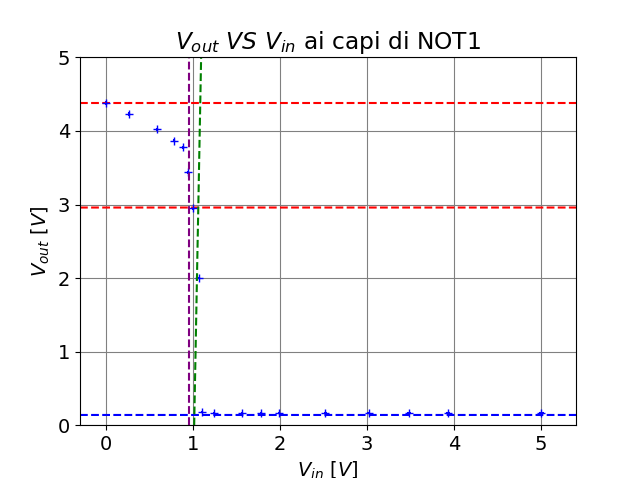
\includegraphics[scale=0.50]{../Figs-Tabs/in-ot2.png}
			\caption{Rappresentazione dei dati in \tablename{ \ref{t:1}}.}
			\label{f:i1}
		\end{figure}
	\end{center}

	
\section{Montaggio arduino}
	Per la verifica delle caratteristiche dinamiche dell'IC SN74LS244 si è montato un circito impulsatore, basato su di un microcontrollore arduino; successivamente impiegato come generatore di onde. 
	
	Si riporta lo schema circitale in \figurename{ \ref{f:impulsatore}}. 
	
		\begin{figure}[htb]
			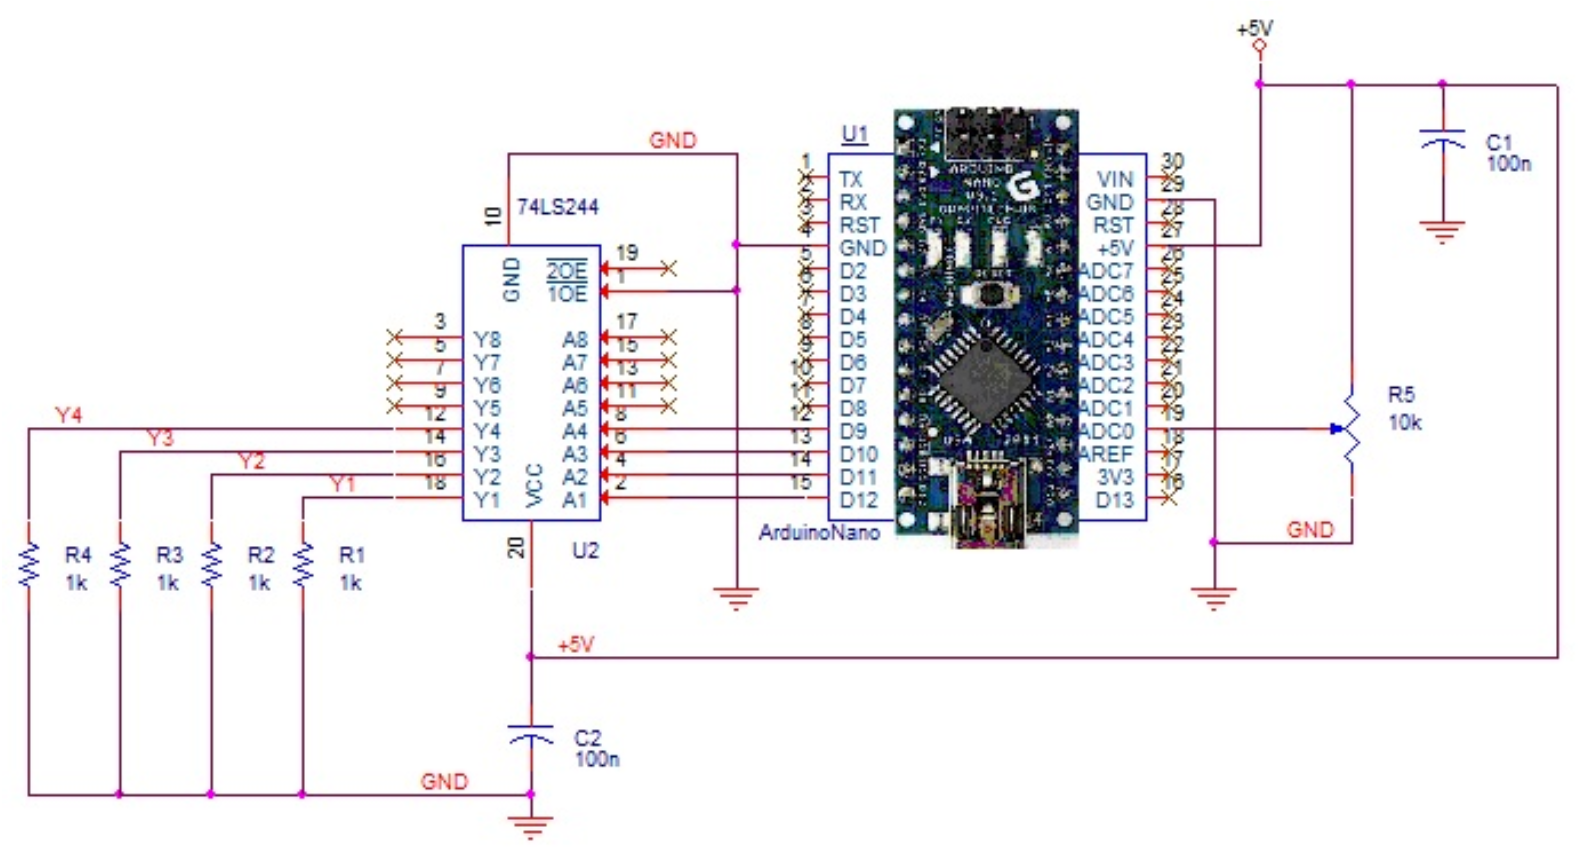
\includegraphics[scale=0.50]{../Figs-Tabs/imp.png}
			\caption{Rappresentazione del circuito impulsatore montato.}
			\label{f:impulsatore}
		\end{figure}
	Per il montaggio sono state impiegate le  segenti componenti circitali:
	\begin{center}
	\bigskip
		$R_{1}=$\SI{984 \pm 8}{\ohm} $R_{2}=$\SI{984 \pm 8}{\ohm} $R_{3}=$\SI{982 \pm 8}{\ohm} \\
		$R_{4}=$\SI{983 \pm 8}{\ohm} n trimmer di $R_{5}^{max}=$\SI{10.2 \pm 0.8}{\kilo \ohm} \\
 		dei condensatori	$C_{1}=$\SI{114 \pm 6 e-9}{\farad} $C_{2}=$\SI{114  \pm 6 e-9}{\farad}
	
	\end{center}
	Si segnala inoltre 
	che da questa sezione si è impiegata una tensione di alimentazione $V_{cc}=$\SI{4.87 \pm 0.03}{\volt}; tale accorgimento è stato impiegato per evitare di danneggiare il microcontrollore arduino, sensibile per tensioni superiori a \SI{5}{\volt}.

	Il circuito montato tra i terminali Y1 e Y2 dovrebbe generare delle onde quadre sfasate di $\pi/2$ , di frequenza regolabile attraverso il valore di $R_{5}$, e  compresa tra 50 Hz e 50KHz.
	
	Si è andati pertanto a verificarne il corretto montaggio attraverso la verifica di queste proprietà.
	Attraverso l'oscilloscopio si sono visalizzati su ch1 la tensione rilevata su Y1 e su  ch2 la tensione letta su Y2. Si riporta una tipica acquisizione in 
	\figurename{ \ref{f:oscil} }.
	\begin{figure}[htb]
		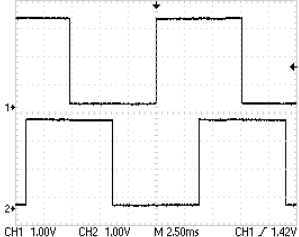
\includegraphics[scale=0.50]{../Figs-Tabs/ondaquadra_esempio.png}
		\caption{Tipica acqisizione delle tensioni lette si terminali Y1 (ch1) e Y2 (ch2) del circuito impulsatore.}
		\label{f:oscil}
	\end{figure}

	Come è possibile osservare dall'acquisizione la forma d'onda presentata dalle due tracce può essere trattata quale un onda quadra; si osserva inoltre che al variare del valore della resistenza $R_{5}$ la frequenza delle tracce assume valori compresi nell'intervallo $f\in [\sim 10 \text{Hz;} \sim 50 \text{KHz}]$.
	
	Come ultima verifica dell'operatività del circuito montato si e proceduto a misurare lo sfasamento tra le due tracce.
	Per fare ciò si è andati a misurare il $\Delta t$ tra i fronti di salita delle dei due canali, ottenendo $\Delta t=$\SI{248 \pm 2}{\mu \sec}\footnote{misura effettuata con i cursori dell'oscilloscopio in dotazione.} a fronte di una frequenza
	  $f=$\SI{1.007 \pm 0.001}{\kilo \hertz}\footnote{la misura di frequenza è stata effettuata con la funzione di lettura automatica dell'oscilloscopio; a cui abbiamo abbiamo associato l'incertezza di un digit sulla cifra precedente alla prima che risultasse instabile. } .
	Essendo valida la relazione \begin{equation}
	\Delta \phi = 2 \pi \cdot f \cdot \Delta t
	\end{equation}\label{eq:sfas}
	si ottiene $\Delta \phi=$\SI{1.57 \pm 0.01 }{\radian} ,compatibile con $\phi/2$.
	
	Visto l'accordo tra le richieste operative ed il funzionamento del circuito impulsatore montato 
	si è assunto  come  corretta la realizzazione dello stesso.
	

\section{Divisori di frequenza}
\subsection{Montaggio e verifica}
Si è innanzitutto realizzato il circuito in \fig{div} utilizzando l'integrato SN74LS93 (un ripple counter costituito da quattro JK flip-flop), mettendo uno degli ingressi di reset ($R_{0,1}$) a terra, per poi verificarne visivamente il corretto funzionamento inviando un clock lento ($\sim \SI{1}{\Hz}$) ed osservando i LED (e dunque gli output dei flip-flop) ``contare'' ciclicamente da 0 a 15.

\begin{figure}[h]
	\centering
	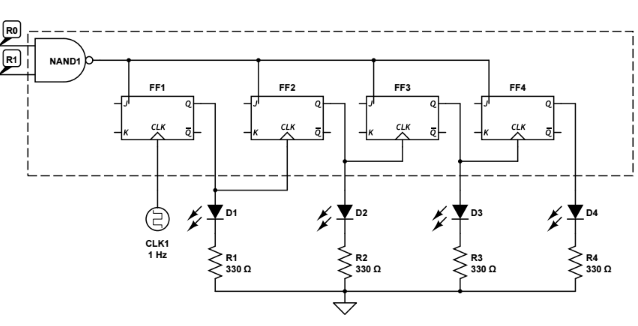
\includegraphics[scale=0.8]{divisori.png}
	\caption{Circuito divisore}
	\label{fig:div}
\end{figure}

\subsection{Verifica funzionamento divisore e misura dei tempi di ritardo.}
Effettuata la verifica precedente si è posta $f_{clock} = \SI{49.998(1)}{ \kilo \hertz}$\footnote{\label{fn:frmeas}Tutte le misure di frequenza sono state eseguite con il frequenzimetro dell'oscilloscopio per via della sua grande precisione; si è preso fino all'ultima cifra stabile con il corrispondente errore.} per procedere dunque alla misura della frequenza dei segnali in uscita ai flip-flop del contatore, ottenendo i valori in \tab{divlag}.

I segnali sono riportati in \fig{divout}. Si ha dunque come atteso un funzionamento da divisore di frequenza (con ottima precisione).

\begin{figure}[h]
	\centering
	\begin{minipage}{0.47\textwidth}
		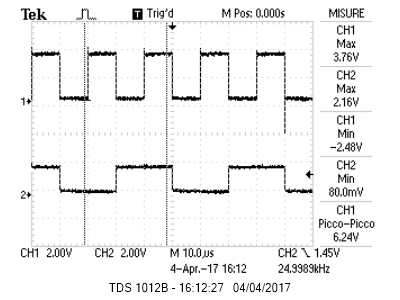
\includegraphics[scale=0.8]{divisore_2x.png}
		\\
		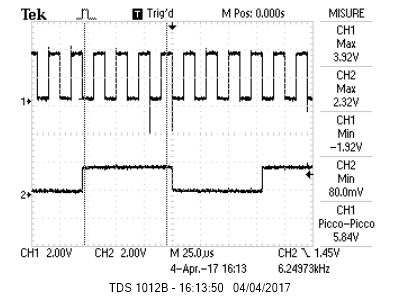
\includegraphics[scale=0.8]{divisore_8x.png}
	\end{minipage}
	\begin{minipage}{0.47\textwidth}
		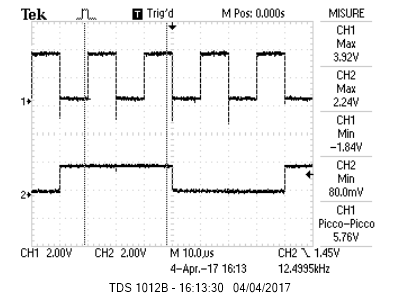
\includegraphics[scale=0.8]{divisore_4x.png}
		\\
		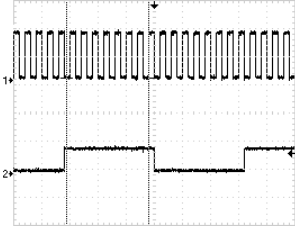
\includegraphics[scale=0.8]{divisore_16x.png}
	\end{minipage}
	\caption{Output dei quattro flip-flop del divisore (CH2) e segnale di clock (CH1).}
	\label{fig:divout}
\end{figure}

Si sono successivamente misurati\footnote{La misura è stata eseguita mediante i cursori dell'oscilloscopio.} i tempi di ritardo degli output dei flip-flop, ovvero l'intervallo temporale tra il fronte (di discesa) del clock in cui ci si attende una variazione dell'output e il fronte della variazione stessa, misurato tra i punti di tensione intermedia tra il livello alto e quello basso. I valori ottenuti sono riportati in \tab{divlag}. %qualquadra non cosa, non riesco a fargli fare la formattazione SI

\begin{table}[h]
	\centering
	\begin{tabular}{l S[table-figures-decimal=4, table-figures-uncertainty=1] S[table-figures-decimal=1, table-figures-integer=3, table-figures-uncertainty=1] S[table-figures-decimal=1, table-figures-uncertainty=1] }
		\toprule
			& {$f$ [\si{\kHz}]} & {$\Delta t_{salita}$ [\si{\ns}]} & {$\Delta t_{discesa}$ [\si{\ns}]} \\
		\midrule
		$Q_1$ & 24.999(1) & 76.0(4) & 24.2(1) \\
		$Q_2$ & 12.499(1) & 101 (1) & 30.8(2) \\
		$Q_3$ & 6.2497(1) & 110 (1) & 42.0(2) \\
		$Q_4$ & 3.1251(1) & 155 (1) & 53.2(4) \\
		\bottomrule
	\end{tabular}
	\caption{Tempi di ritardo e frequenze misurate per il circuito divisore.}
	\label{tab:divlag}
\end{table}

Come atteso, il ritardo è maggiore per i flip-flop più ``a valle'', dal momento che il segnale deve propagarsi attraverso tutti i flip-flop precedenti.

\paragraph{Divisore 10x, circuito di reset}
Per ottenere dal contatore un segnale di frequenza pari a 1/10 di quella del clock è stato deciso di implementare un circuito di reset sincrono, riportato in \fig{reset}: si usa l'output del primo e del quarto flip-flop come ``flag'' di reset, dimodoché esso avvenga al colpo di clock successivo al raggiungimento del 9 binario (sul fronte di discesa, come per il resto dei cambi di stato, essendo questo il fronte a cui sono sensibili i flip-flop del contatore), completando dunque un ciclo di 10 periodi di clock.
Più dettagliatamente, quando il contatore raggiunge il 9 (necessariamente su un fronte di discesa del clock), l'output della prima NAND diventa 0, ma il D-Latch a cui esso è collegato resta disabilitato fino alla risalita del clock; con la risalita il D-Latch può cambiare stato seguendo l'input ed il suo output $\overline{Q}$ pasa da 0 a 1, la NAND di Clear dell'integrato resta però bloccata dall'altro suo input (il clock negato, che è dunque basso in questo momento): al fronte di discesa del clock, quando il contatore dovrebbe passare da 9 a 10, essa finalmente cambia stato, resettando il contatore a 0 (e il D-Latch resta bloccato, in modo da avere un segnale di Clear stabile per mezzo periodo di clock nonostante la variazione degli output $Q_1$ e $Q_4$).

\begin{figure}[h]
	\centering
	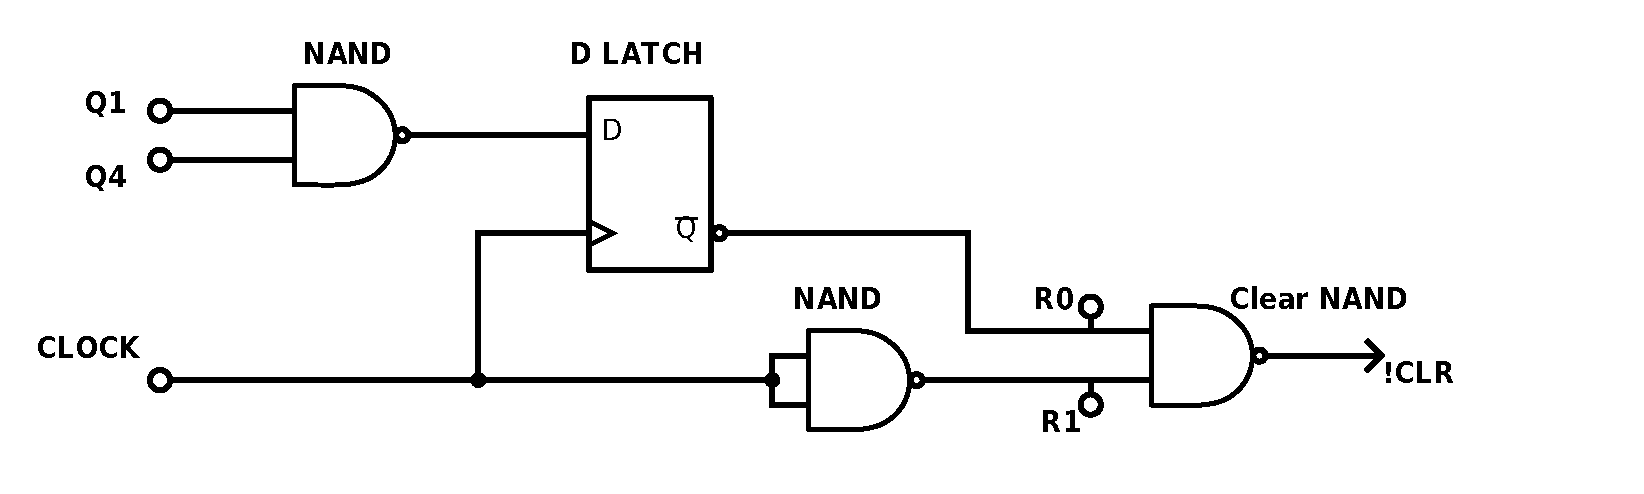
\includegraphics{resetter.pdf}
	\caption{Circuito di reset per il contatore.}
	\label{fig:reset}
\end{figure}

Il D-Latch usato nel circuito di reset è quello realizzato nella sezione precedente dell'esercitazione, sono inoltre state utilizzate altre due porte NAND (la terza è contenuta nell'integrato stesso, con ingressi alle porte 2 e 3). Utilizzare l'output $\overline{Q}$ del D-Latch ci consente di risparmiare una porta NAND, altrimenti necessaria per invertire l'output della prima NAND (l'input del D-Latch).

Il risultato è visibile \fig{div10}, dove qualitativamente si può notare come il segnale in uscita al flip-flop più significativo abbia un periodo pari a 10 periodi di clock (si è anche verificato visivamente attraverso i LED che il comportamento fosse quello atteso); quantitativamente, con un clock a frequenza $f_{clock} = \SI{49.998(1)}{ \kilo \hertz}$ (lo stesso utilizzato nelle misure precedenti) si ottiene in uscita un segnale di frequenza $f_{4} = \SI{4.9999(1)}{ \kilo \hertz}$\fn{frmeas}.

\begin{figure}[h]
	\centering
	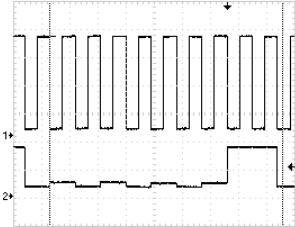
\includegraphics{divisore_10x.bmp}
	\caption{Segnale in uscita al quarto flip-flop del contatore in configurazione divisore 10x.}
	\label{fig:div10}
\end{figure}

\section{Multivibratore astabile}
Si è montato il circuito in \fig{astab_sch}, con i seguenti valori dei componenti:

\begin{figure}[H]
	\begin{minipage}{0.8\textwidth}
		\centering
		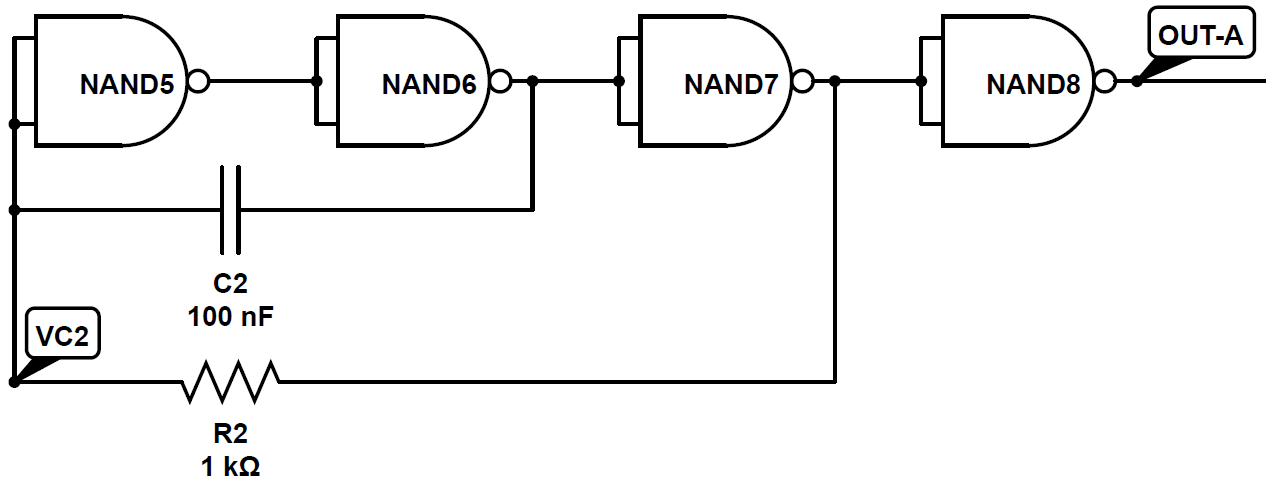
\includegraphics[scale=0.35]{astabile.png}
		\caption{Multivibratore astabile}
		\label{astab_sch}
	\end{minipage}
	\begin{minipage}{0.1\textwidth}
		\begin{tabular}{l}
			$R_2 = \SI{982(8)}{\ohm}$\\
			$C_2 = \SI{109(4)}{\nano \farad}$
		\end{tabular}
	\end{minipage}
\end{figure}

Si è verificato che il segnale in uscita fosse un onda quadra, come visibile in \fig{astab_osc} e si sono misurati periodo è duty cycle, che risultano valere:
$$T = \SI{204(1)}{\micro \second} \qquad D\% = \SI{70.1(6)}{\%}$$

\begin{figure}[H]
	\centering
	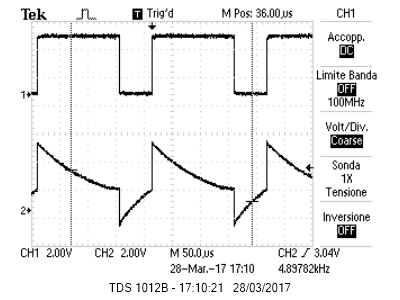
\includegraphics[scale=1]{astabile_inout.png}
	\caption{OUT-A e VC2 del multivibratore astabile}
	\label{astab_osc}
\end{figure}

Si è quindi andati ad osservare la forma d'onda all'ingresso del primo NAND (VC2), come visibile nella stessa \fig{astab_osc}.
La tensione oscilla tra \SI{4.48(12)}{\volt} e \SI{-0.68(2)}{\volt}, mentre la commutazione avviene a \SI{1.44(4)}{\volt}.

\subsection{Analisi del funzionamento}

Consideriamo un istante prima della commutazione basso/alto del NAND6 (o equivalentemente sull'uscita OUT-A): VC2 si appresta a superare $V_{comm}=\SI{1.44}{\volt}$ (la tensione di commutazione) e, essendo l'uscita del NAND6 bassa, la tensione sul condensatore è proprio uguale a VC2 ($\Delta V_C = VC_2 - V_{NAND6}$).

Raggiunta la tensione di commutazione l'uscita del NAND6 viene forzata allo stato HIGH e l'uscita del NAND7 si troverà in stato LOW, questo aumenterà istantaneamente la tensione VC2 di $V_{HIGH}=\sim \SI{3.04}{\volt}$, pari alla tensione dello stato HIGH della porta logica. Da questo punto in poi il condensatore si scaricherà con un $\tau = RC$, fino a raggiungere nuovamente la tensione di commutazione.

Nel passaggio alto/basso del NAND6 la situazione è diversa: VC2 dal valore di $\sim \SI{1.44}{\volt}$ non può diminuire oltre i $\sim\SI{-0.7}{\volt}$ per la presenza di diodi di protezione agli ingressi delle porte logiche, a questo è dovuta l'asimmetria dei semiperiodi.

Il semiperiodo HIGH è atteso essere pari a $RC\times \ln(V_{HIGH}/V_{comm}) = \SI{122(5)}{\micro\second}$, non compatibile con quello misurato di \SI{143(1)}{\micro\second}, il motivo è da ricercarsi probabilmente nel fatto che l'uscita del NAND6 non appariva costante ma aumentava leggermente nel corso del semiperiodo.
	
\subsection{Linearità del periodo con la resistenza}
Si è variata la resistenza $R_2$ in un intorno di $\SI{1000}{\ohm}$ e per ogni valore di resistenza di è misurato il periodo del segnale. I risultati raccolti sono riportati in appendice in \tab{astab_data}.
Si è quindi proceduto ad un fit lineare ($ax+b$), ottenendo i seguenti risultati:
$$a = \SI{20.74(27)}{\ohm / \micro\second} \qquad b=\SI{1.6 \pm 2.5}{\micro \second} \qquad \chi^2/ndof = 10.7/7 \qquad corr(a,b)= -0.966$$
In \fig{astab_lin} sono rappresentati i dati raccolti e il fit eseguito.

\begin{figure}[h!]
	\centering
	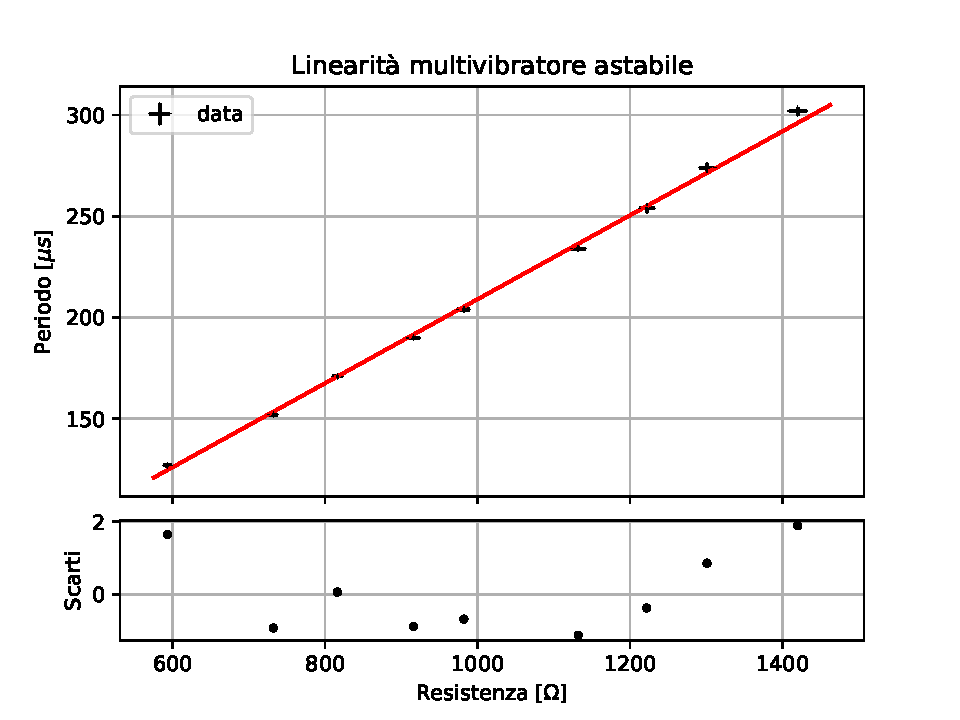
\includegraphics[scale=0.9]{fit_dati_3.pdf}
	\caption{Dati raccolti e fit della linearità del multivibratore astabile}
	\label{astab_lin}
\end{figure}




	\end{document}
